\section{Динамические фильтры}

\subsection{Постановка задачи}
В соответствии с заданием рассмотрим прямоугольный импульс, заданный параметрами $a = 4$, $t_1 = -17$, $t_2 = 27$:
\begin{equation*}
    g(t) =
    \begin{cases}
        4, & t \in [-17, 27],    \\
        0, & t \notin [-17, 27].
    \end{cases}
    \label{eq:gt}
\end{equation*}
Зашумлённая версия сигнала имеет вид:
\begin{equation*}
    u(t) = g(t) + b\xi(t) + c\sin(dt),
    \label{eq:ut}
\end{equation*}
где $\xi(t) \sim U[-1, 1]$ - белый шум с равномерным распределением, а $b, c, d$ - параметры возмущения. Для анализа сигналов используем унитарное преобразование Фурье по угловой частоте $\omega$:
\begin{equation*}
    \hat{u}(\omega) = \frac{1}{\sqrt{2\pi}} \int_{-\infty}^{\infty} u(t) e^{-i\omega t} \, dt, \quad
    u(t) = \frac{1}{\sqrt{2\pi}} \int_{-\infty}^{\infty} \hat{u}(\omega) e^{i\omega t} \, d\omega.
    \label{eq:ft}
\end{equation*}

\subsection{Фильтр первого порядка}
Примем $c = 0$, тогда сигнал содержит только полезную составляющую и белый шум: $u(t) = g(t) + b\xi(t)$. Пропустим его через линейный динамический фильтр первого порядка с передаточной функцией
\begin{equation*}
    W_1(p) = \frac{1}{Tp + 1},
    \label{eq:w1}
\end{equation*}
где $T > 0$ - постоянная времени фильтра.\\

Давайте сравним графики исходного и зашумлённого сигналов. Выберем для этого $T=2$ и $b=0.5$

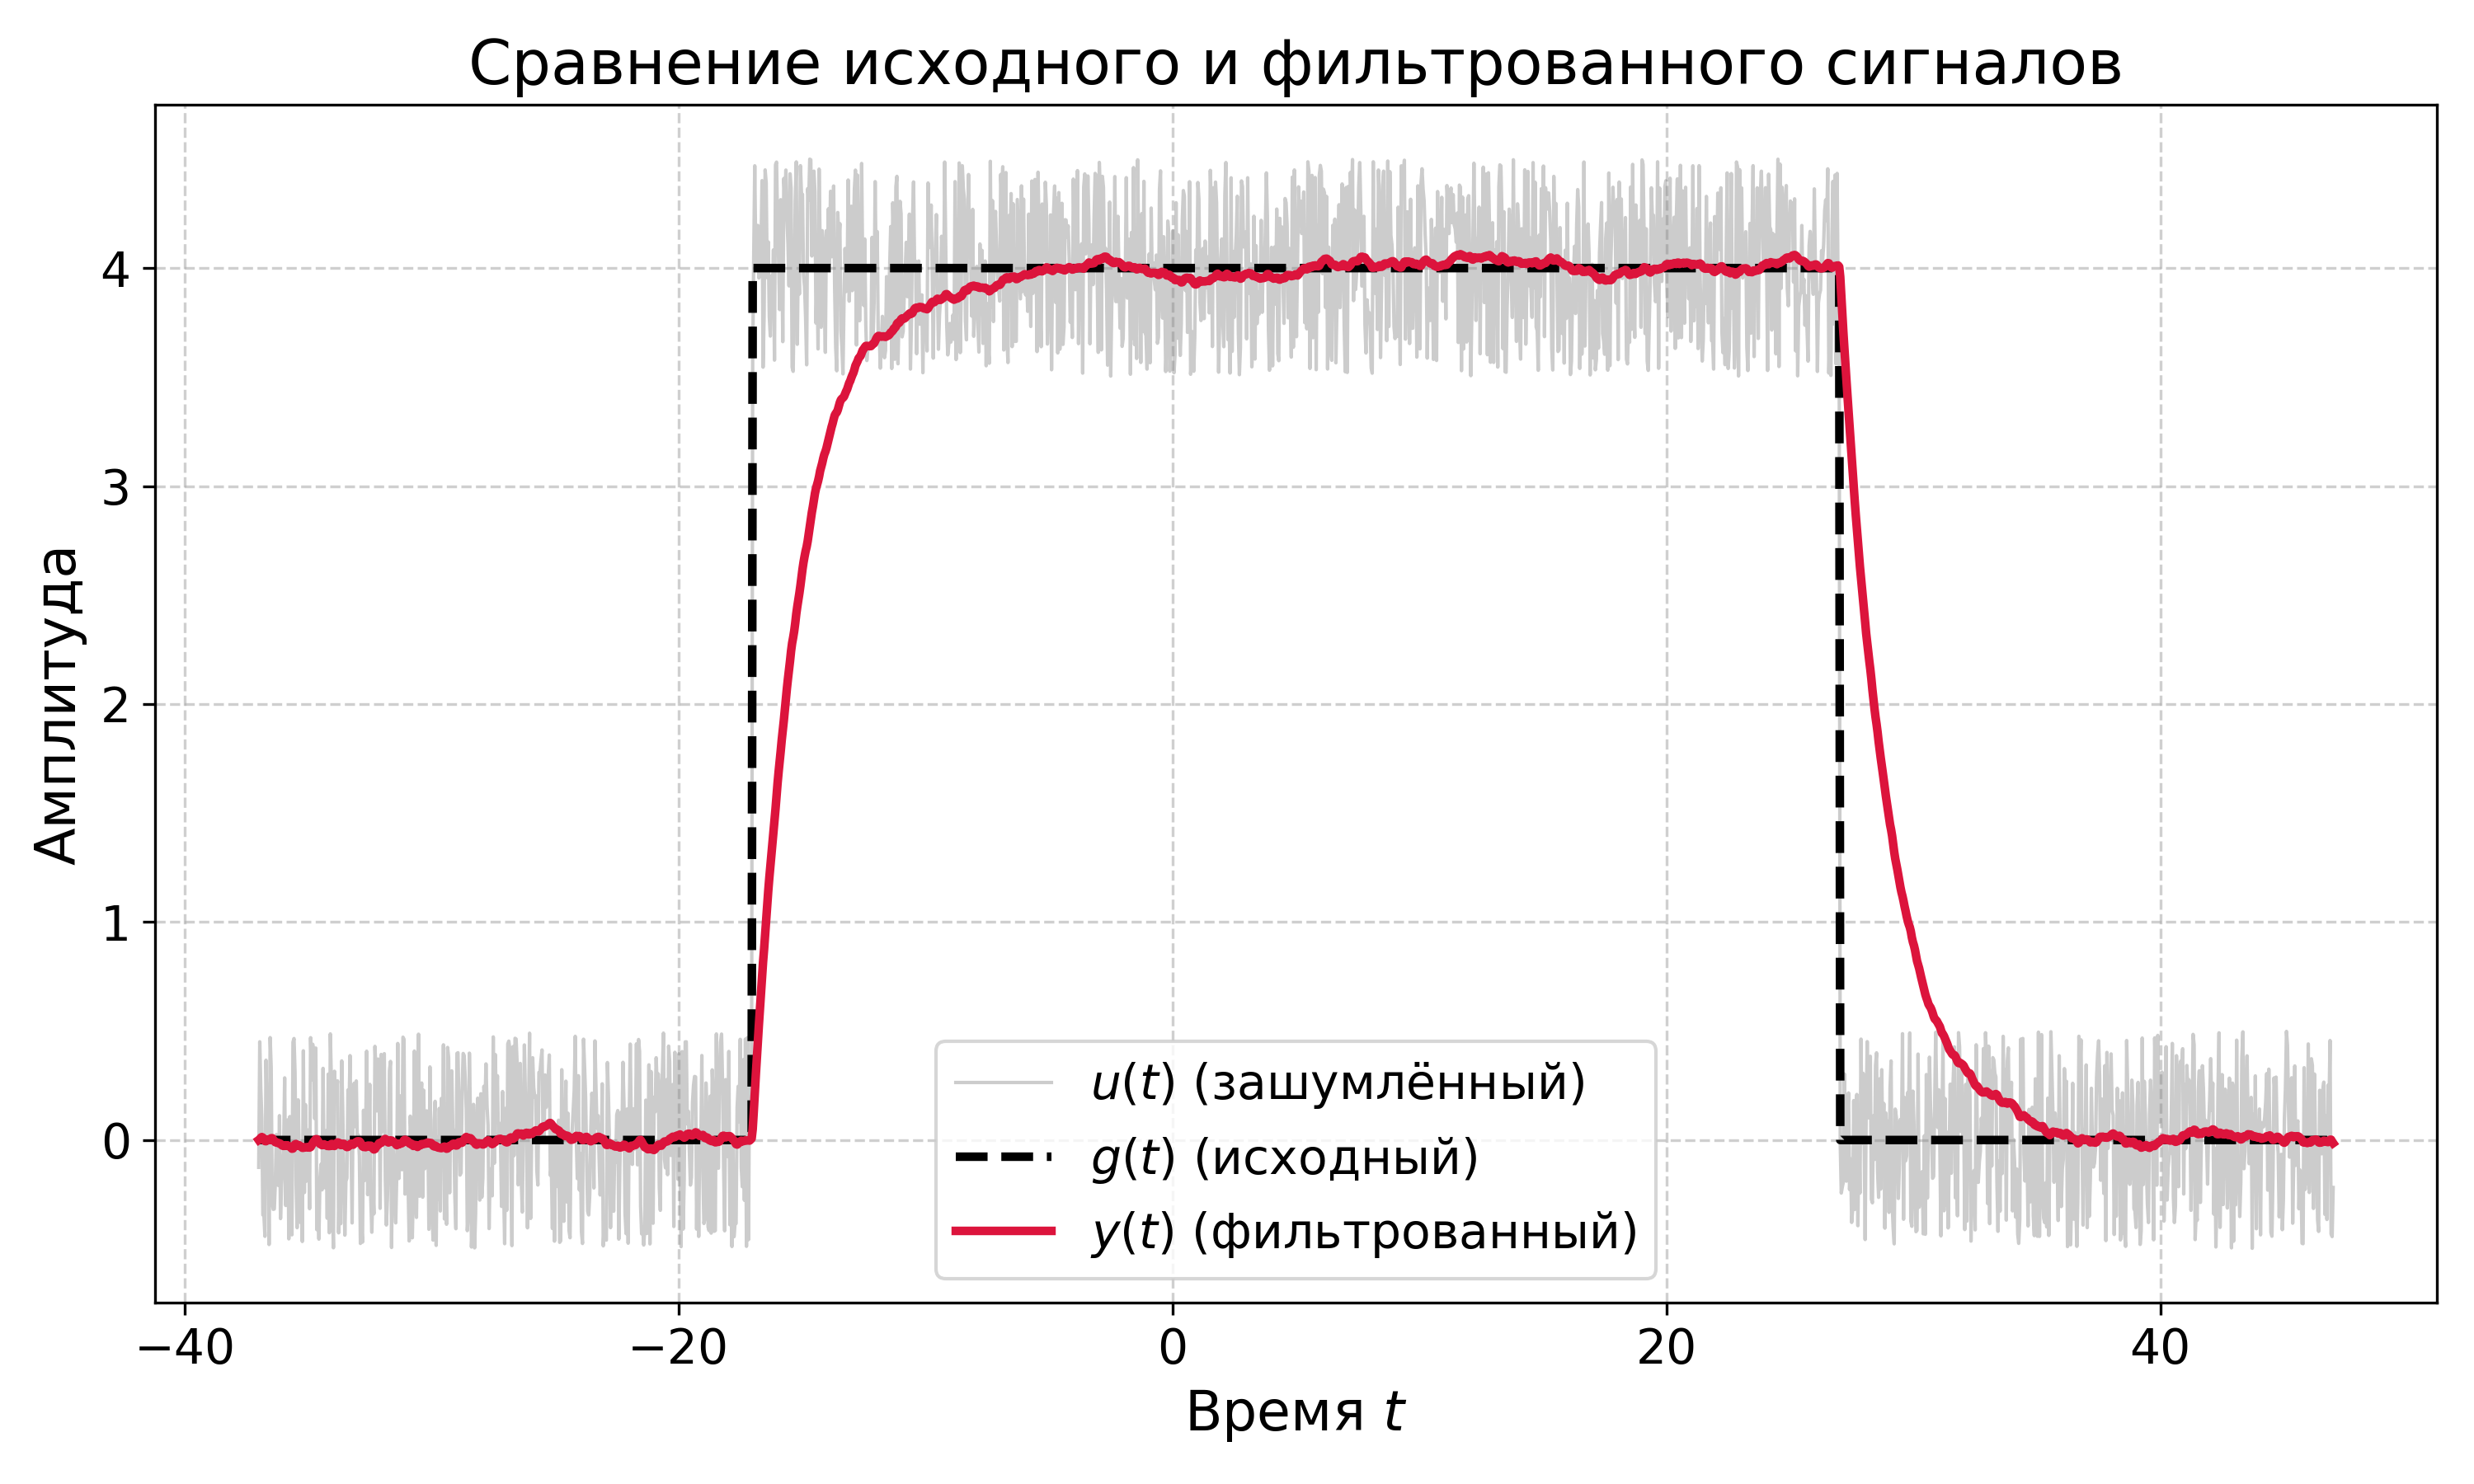
\includegraphics[width=\textwidth]{images/1_4/first_comparison_of_signals.png}

